\setAuthor{Ardi Loot}
\setRound{lahtine}
\setYear{2019}
\setNumber{G 6}
\setDifficulty{6}
\setTopic{TODO}

\prob{Led}
\begin{wrapfigure}[7]{r}{0.5\textwidth}
	\vspace{-24pt}
	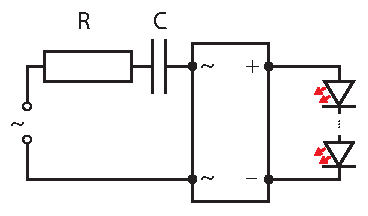
\includegraphics[width=0.5\textwidth]{2019-lahg-06-yl.pdf}
\end{wrapfigure}

LED-lamp koosneb $N=10$-st valgusdioodist (nimipinge $U_{D}=\SI{3.0}{V}$ ja -vool $I_{D}=\SI{100}{mA}$), mida toidetakse vahelduvvooluga (pinge maksimumväärtus $U=\SI{320}{V}$ ja sagedus $f=\SI{50}{Hz}$) läbi takisti ($R=\SI{400}{\ohm}$), kondensaatori ja alaldi (lugeda ideaalseks). Kui suur peab olema kondensaatori mahtuvus $C,$ et valgusdioodid põleksid võimalikult heledalt, kuid ei põleks läbi? Märkus: Takisti ja kondensaatori näivtakistus on $Z=\sqrt{R^{2}+X_{C}^{2}}$, kus $X_{C}=1/\left(2\pi fC\right)$ ning võib eeldada sinusoidaalset voolu ja pinget aladi ees. 


\hint

\solu
Valgusdioodid põlevad võimalikult heledalt, ja ei põle läbi, nimipingel
ja voolul. Pinge jaotumise kohta saab kirja panna võrrandi $U=I_{D}Z+NU_{D}$
ja seda lahendades leida vajaliku takisti ja kondensaatori näivtakistuse 
\begin{equation*}
Z=\frac{U-NU_{D}}{I_{D}}=\SI{2.9}{k\Omega}.
\end{equation*}
Kasutades takisti ja kondensaatori näivtakistuse valemit saame avaldada
vajaliku mahtuvuse
\begin{equation*}
C=\frac{1}{2\pi f\sqrt{Z^{2}-R^{2}}}\approx\SI{1.1}{\mu F}.
\end{equation*}
\probend